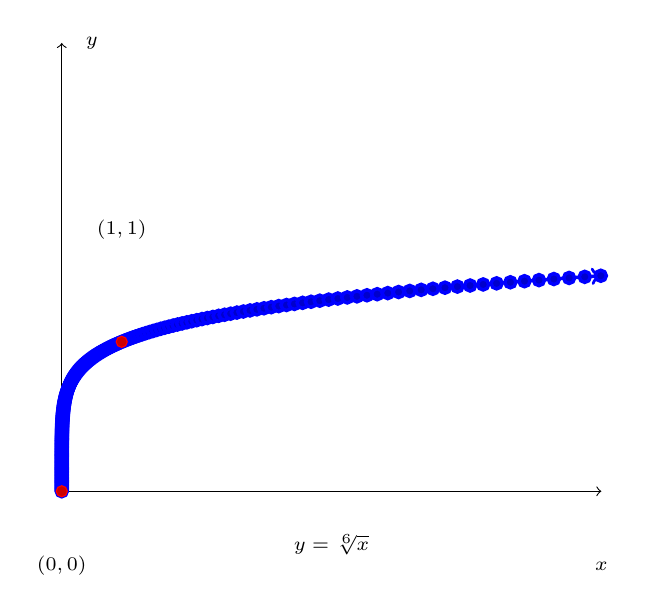
\begin{tikzpicture}
\begin{axis}[
  xmin=0, xmax=9,
  ymin=0, ymax=3,
  axis lines=middle,
  axis line style={->},
  ticks=none,
  clip=false
]
\node at (axis cs:9,-0.5){\scriptsize $x$};
\node at (axis cs:0.5,3){\scriptsize $y$};
\node at (axis cs:1,1.75){\scriptsize $(1,1)$};
\node at (axis cs:0,-0.5){\scriptsize $(0,0)$};

\addplot+[domain=0:1.442, samples=200, smooth, line width=1.25pt, ->, variable=\t, parametric]
  ({\t^6},{\t});

\addplot+[only marks, mark=*, mark size=2pt] coordinates {(0,0) (1,1)};

% Caption
\node at (rel axis cs:0.5,-0.12){\scriptsize $y=\sqrt[6]{x}$};
\end{axis}
\end{tikzpicture}